\documentclass[a4paper, 11pt]{report}
\usepackage{blindtext}
\usepackage[T1]{fontenc}
\usepackage[utf8]{inputenc}
\usepackage{titlesec}
\usepackage{fancyhdr}
\usepackage{geometry}
\usepackage{fix-cm}
\usepackage[hidelinks]{hyperref}
\usepackage{graphicx}
\usepackage{titlesec}

\usepackage[english]{babel}

\geometry{ margin=30mm }
\counterwithin{subsection}{section}
\renewcommand\thesection{\arabic{section}.}
\renewcommand\thesubsection{\thesection\arabic{subsection}.}
\usepackage{tocloft}
\renewcommand{\cftchapleader}{\cftdotfill{\cftdotsep}}
\renewcommand{\cftsecleader}{\cftdotfill{\cftdotsep}}
\setlength{\cftsecindent}{2.2em}
\setlength{\cftsubsecindent}{4.2em}
\setlength{\cftsecnumwidth}{2em}
\setlength{\cftsubsecnumwidth}{2.5em}

\titlespacing\section{0pt}{12pt plus 4pt minus 2pt}{0pt plus 2pt minus 2pt}
\titlespacing\subsection{0pt}{12pt plus 4pt minus 2pt}{0pt plus 2pt minus 2pt}

\begin{document}
\titleformat{\section}
{\normalfont\fontsize{15}{0}\bfseries}{\thesection}{1em}{}
\titlespacing{\section}{0cm}{0.5cm}{0.15cm}
\titleformat{\subsection}
{\normalfont\fontsize{13}{0}\bfseries}{\thesubsection}{0.5em}{}
\titlespacing{\section}{0cm}{0.5cm}{0.15cm}

%=============================================================================

\pagenumbering{Alph}
\begin{titlepage}
\begin{flushright}

\includegraphics[width=4cm]{Images/USyd.jpg}\\[2cm]
\end{flushright}
\center 
\textbf{\huge INFO1111: Computing 1A Professionalism}\\[0.75cm]
\textbf{\huge 2023 Semester 1}\\[2cm]
\textbf{\huge Self-Learning Report}\\[3cm]

\textbf{\huge Submission number: 1}\\[0.75cm]
\textbf{Github link: ??}\\[2cm]

{\large
\begin{tabular}{|p{0.35\textwidth}|p{0.55\textwidth}|}
	\hline
	{\bf Student name} & Deana Hamdan El Madi\\
	{\bf Student ID} & 520481770\\
	{\bf Topic} & JavaScript\\
	{\bf Levels already achieved} & -\\
	{\bf Levels in this report} & A and B \\
	\hline
\end{tabular}
}
\thispagestyle{empty}
\end{titlepage}
\pagenumbering{arabic}


%=============================================================================

\tableofcontents

%=============================================================================


\newpage
\section{Level A: Initial Understanding}
\vspace{5mm}
\subsection{Level A Demonstration}
To demonstrate my Level A understanding of JavaScript, I will:

- Embed JavaScript into a web-page

- Create functions in JavaScript

- Learn about scope in JavaScript


\subsection{Learning Approach}
I approached my learning by first seeking to understand the fundamentals of JavaScript. This included basic syntax, data types and control structures. An important step in my learning approach was to cultivate good habits, such as commenting my code and writing clear and concise functions. I sought a demonstration of this by experienced developers, to ensure I was using best practise in my work. 
I browsed various resources to find a teaching style I liked. Through this, I stumbled across "Frontend Simplified" which taught how JavaScript is applied in Frontend Development. Since I was only a beginner, I started by watching the JavaScript crash-course.
I also joined Frontend Simplified's programming Discord server. This proved to be a very useful step in my self-learning journey, as participating in an online community allowed me to ask questions and learn from other people. I was able to find mentors and accountability partners to help me stay on track as I navigated through the content.
The final element of my learning approach was to be patient. I understood that learning a new language takes time and effort. I tried to not get discouraged if I didn't understand something right away, and wasn't afraid to ask for help or take a break when I needed it.


\subsection{Challenges and Difficulties}
Embedding JavaScript into a web-page is what I found most difficult, as this is a concept I haven't encountered in other programming languages. I didn't have prior experience in browser coding, or writing code for an interface. Rather than just writing a program in a JavaScript file, I learnt how to add JavaScript code to the HTML code of a web-page so that the browser can interpret and execute the JavaScript code when the web-page loads.

Another challenging concept was scope. This was because there are many factors in JavaScript that affect where a variable can be accessed. Although I had previous knowledge about global and local scope, I was introduce to block scope. The most difficult concept to grasp was "hoisting". This involved variables being used before they are declared! Variable and function declarations are moved (or "hoisted") to the top of their respective scope before any code is executed.


\subsection{Learning Sources}

\begin{tabular}{|p{0.45\textwidth}|p{0.45\textwidth}|}
	\hline
	Learning Source & Contribution to Learning \\
	\hline
	MDN Web Docs\cite{MDN_HTML_JS} JavaScript documentation on how to use JavaScript within a web-page. & Documentation is an essential resource for developers and learners alike, and greatly enhanced my learning process. I used MDN Web Docs to learn the syntax and functionality of writing JavaScript within HTML, explore new features and integrations, and troubleshoot specific problems I encountered.  Additionally, the documentation includes best practices and conventions for writing efficient, clean, and readable code. This helped me write code that is consistent with industry standards and is easy to maintain and understand.\\
	\hline
	Frontend Simplified: JavaScript crash-course \cite{FES_JS_Crash_Course}, JavaScript Beginner Challenges\cite{FES_JS_Beginner}, JavaScript Medium Challenges\cite{FES_JS_Medium}, JavaScript Advanced Challenges\cite{FES_JS_Hard}, JavaScript Interview Questions 
 (Fundamentals) \cite{FES_JS_Interview}& The JavaScript crash-course provided a quick and comprehensive overview of the language syntax and functionality, to help me understand the basics of the language. I used the challenge questions to learn how to create functions in JavaScript and apply what I learnt in a practical way, helping me reinforce my understanding of the language and develop my problem-solving skills. \\
	\hline
	Udemy: The Modern JavaScript Bootcamp\cite{Udemy_JS_Course} & The specific videos I watched from this bootcamp related to variable scoping. JavaScript scoping rules can be complex and confusing, and watching a video on the topic allowed me to see examples in action. The instructor provided examples and demonstrations that help to illustrate the key points.\\
	\hline
\end{tabular}

\subsection{Application artifacts}
I learnt how to embed JavaScript into a web-page using a <script> tag (Figure 1). There is an alternate method of having a separate .js file that is referenced with an src attribute.

In the JavaScript code, I used the \emph{alert()} function. This displays a pop-up dialog box with a message and an OK button. The message can be a string or a variable that contains a string. The alert function is used to provide a quick message or notification to the user and interrupts the execution of the JavaScript code until the OK button is clicked.

I opened my \emph{hello.html} file in my local host, and the dialog box appeared with my message (Figure 2). I was therefore successful in embedding JavaScript in the web-page. 

Additionally, I used the \emph{console.log()} method to write a message to the browser's console (Figure 3). The console is a tool that allows developers to view and interact with the JavaScript code that runs on a web-page. It can be accessed by opening the developer tools in a browser and selecting the "Console" tab.

\begin{figure}[ht]
    \centering
    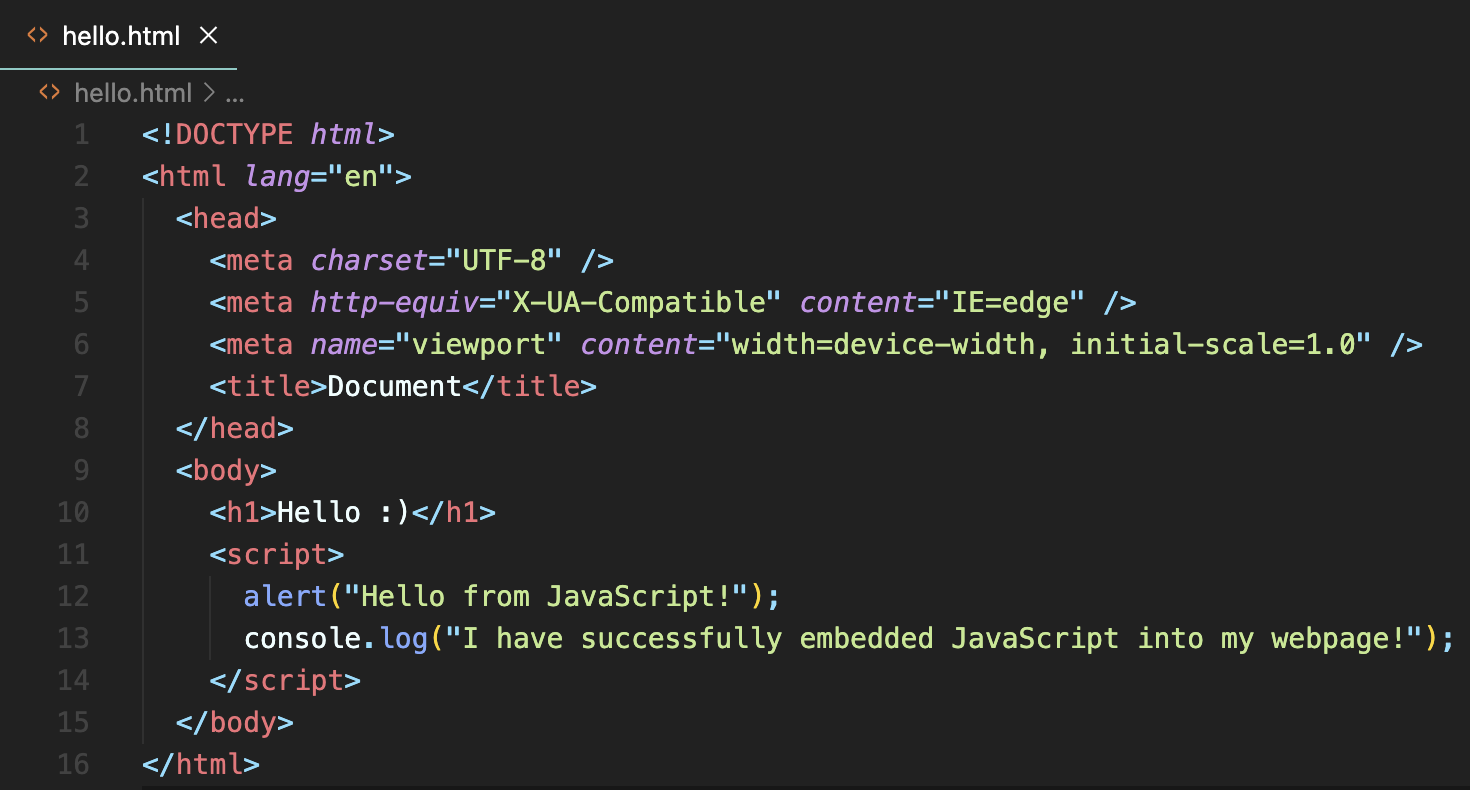
\includegraphics[width=0.8\textwidth]{Images/embedding1.png}
    \caption{Embedding JavaScript into a webpage}
    \label{fig:screenshot}
\end{figure}

\begin{figure}[ht]
    \centering
    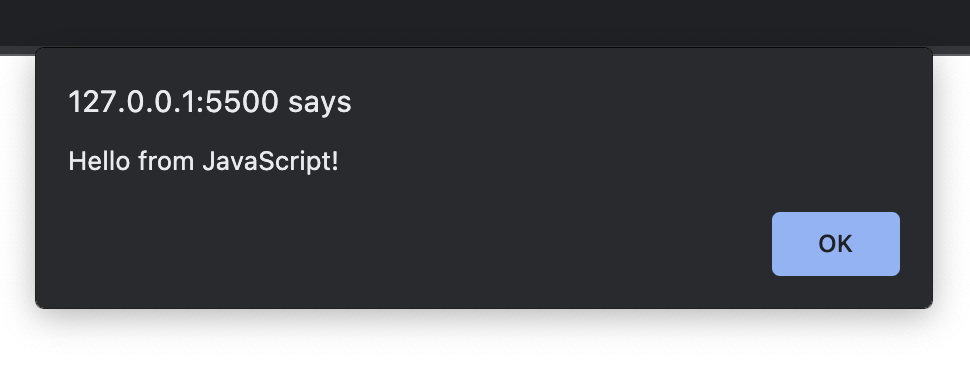
\includegraphics[width=0.8\textwidth]{Images/embedding2.png}
    \caption{Web-page's pop-up dialog box}
    \label{fig:screenshot}
\end{figure}

\begin{figure}[ht]
    \centering
    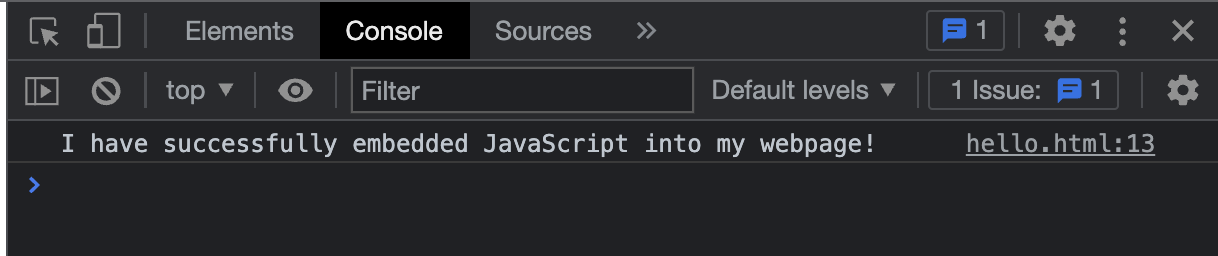
\includegraphics[width=0.5\textwidth]{Images/embedding3.png}
    \caption{Web-page's console}
    \label{fig:screenshot}
\end{figure}

I then sought to learn how to create functions in JavaScript. I started with simple functions that perform basic tasks, such as adding two numbers together or printing a message to the console. This helped me get comfortable with the syntax and structure of functions in JavaScript. After overcoming the basics, I explored more advanced topics, such as function hoisting, closures, and callbacks. These concepts helped me write more powerful and flexible code.

I began solving challenge questions in JavaScript (Figure 4. There are more functions that I created in my GitHub repository in \emph{functions.js}). I was stumped at the start because the challenges required JavaScript methods to solve that I was unaware existed. Every time I looked at a solution and stumbled across a new method, I was forced to research more about it to understand how it is used. 

The function I created in Figure 4 works as follows: Given an array filled with object ID's, the function returns a list of unique ID's in a string. For this problem, I learnt how to use the map method that calls a provided callback function, how to use the JavaScript spread operator, and how to effectively convert an array to string with comma separated values.

The challenge questions helped identify areas where I needed to improve my understanding of the language, allowing me to focus my learning efforts more effectively. Watching a video and completing interactive challenges was an engaging and interactive way to learn, keeping me motivated and interested in the material. By completing challenge questions and seeing my progress, I built confidence in my ability to write JavaScript functions and tackle increasingly complex problems.

\begin{figure}[ht]
    \centering
    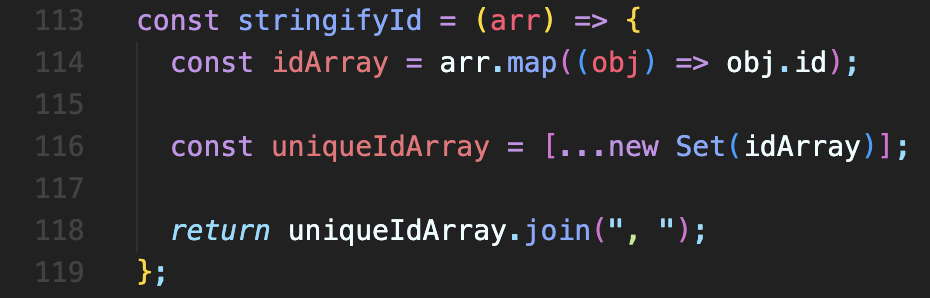
\includegraphics[width=0.5\textwidth]{Images/functions.png}
    \caption{JavaScript challenge question that I solved while learning how to create functions}
    \label{fig:screenshot}
\end{figure}

The final thing left to learn for Level A was scoping. I had covered some of this whilst learning about functions, but sought a more comprehensive understanding of the topic. 

I mainly read documentation and watched videos to understand this concept, and tried different things out myself. I built varying nested structures, and ran my code to see the output in the console. I compiled notes in my \emph{scope.js} file of my findings. Figure 5 shows a snippet of my notes on scope in JavaScript. I investigated Lexical Scoping, Vairable Shadowing and Leaked Globals. 

\begin{figure}[ht]
    \centering
    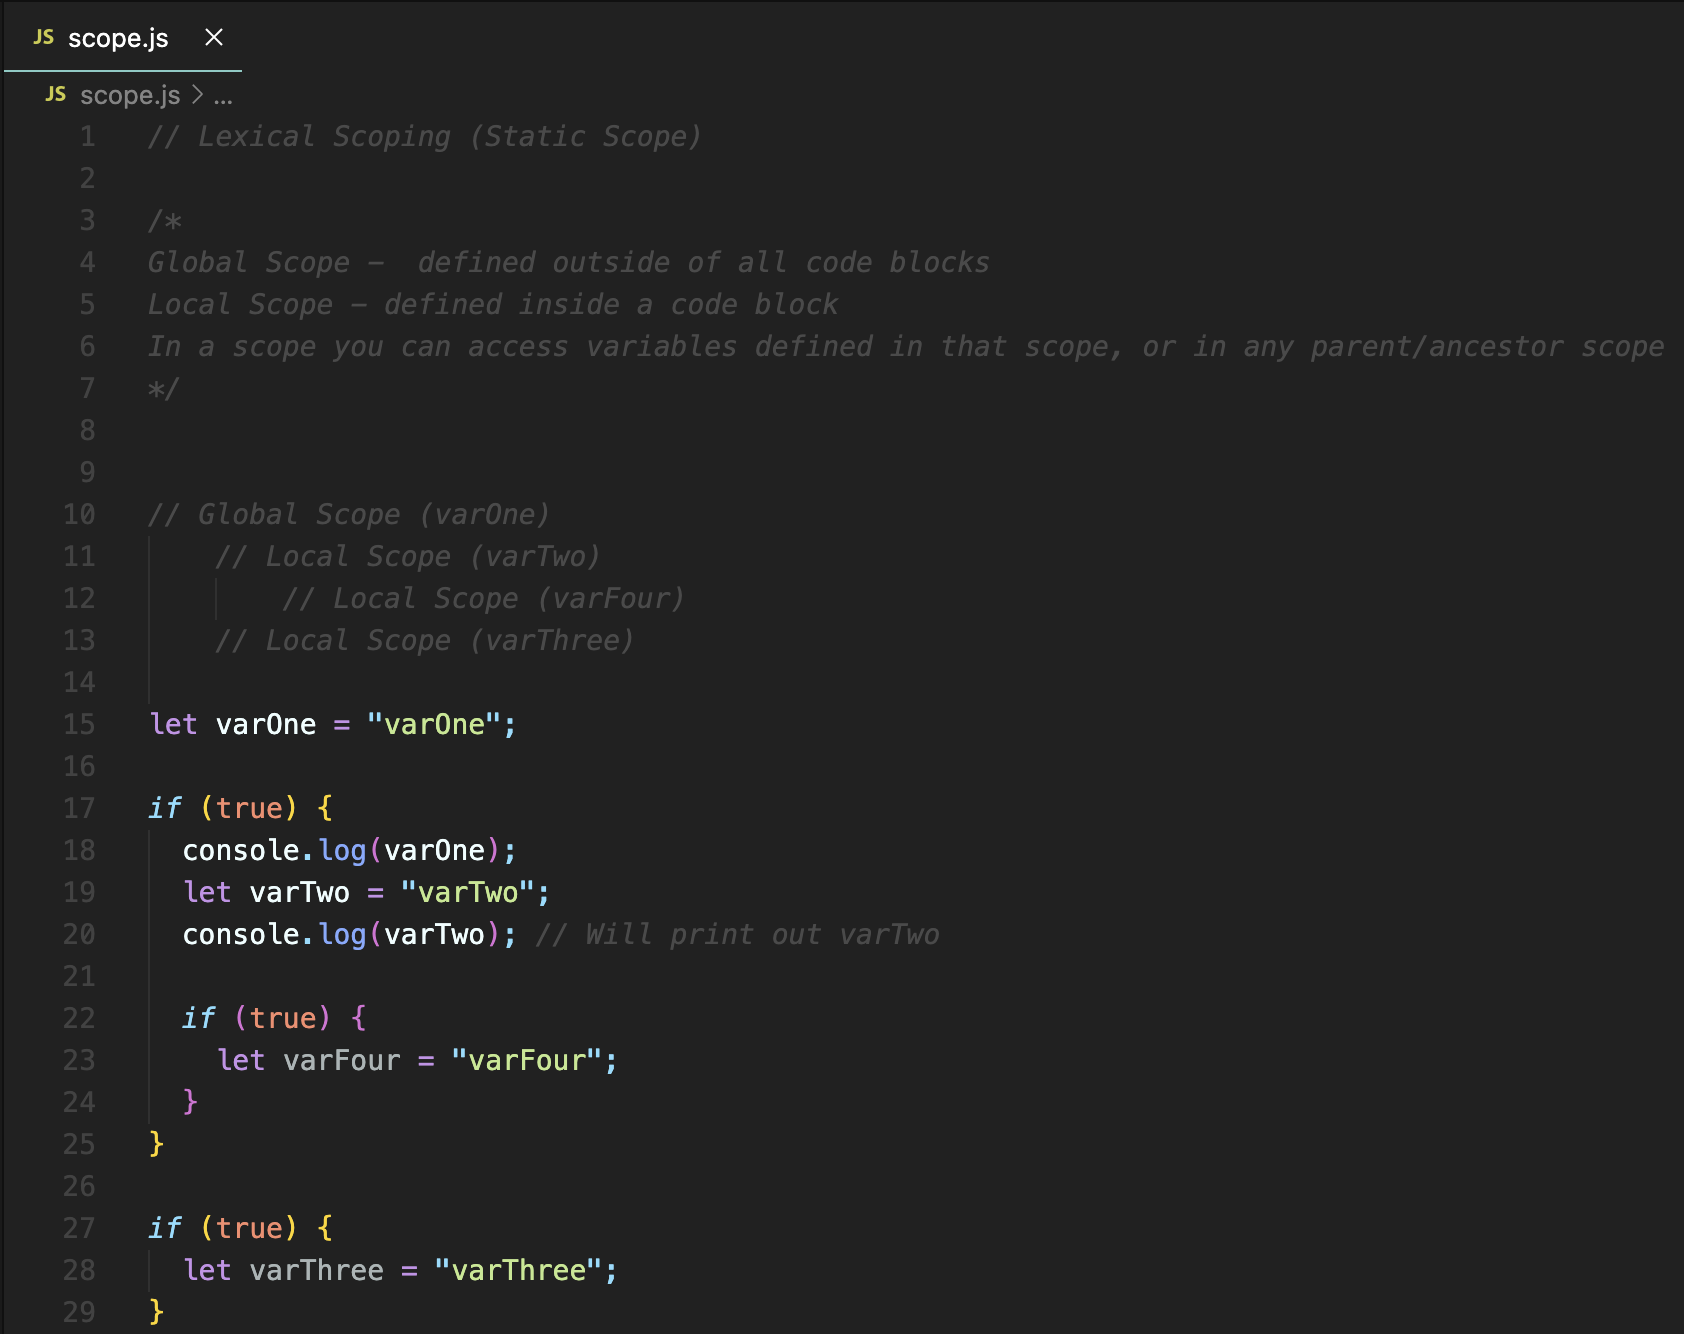
\includegraphics[width=0.8\textwidth]{Images/scope.png}
    \caption{My notes on JavaScript Scope}
    \label{fig:screenshot}
\end{figure}

%=============================================================================

\newpage
\section{Level B: Basic Application}

\subsection{Level B Demonstration}

The key concepts demonstrate for Level B are:

- Embedding JavaScript into a web-page

- JavaScript functions

- Accessing web-page elements

- Event-based triggers

I have incorporated all of these concepts to create a counter. My application involves a HTML structure for the counter, including buttons to increment and decrement the counter and a place to display the current count (embedding JavaScript into a web-page, accessing web-page elements). I added JavaScript code to listen for button clicks and update the counter accordingly (event-based triggers, functions). I added additional CSS to style my counter application.

\subsection{Application artifacts}

I created a simple counter application using JavaScript embedded into a web-page. The application displays the current count on the page and provides three buttons: Increment, Decrement, and Reset. The user can interact with these buttons to manipulate the counter value (Figure 6).

Here's how it works and how I created it:

First I created the basic HTML structure with a heading, a paragraph to display the count, and three buttons with unique id attributes for incrementing, decrementing, and resetting the counter. I was able to access these web-page elements using their id attributes (Figure 7). The JavaScript \emph{getElementById()} returns a reference of the element whose id property matches the specified string. 

I then added JavaScript code by having a separate \emph{app.js} file that is referenced in the HTML code using a <script> tag. JavaScript is required to handle the functionality of the counter.

I initialised a variable \emph{count} to store the current counter value, starting at 0. The function \emph{updateCounterDisplay()} sets the \emph{innerHTML} of the \emph{counterDisplay}y element to the current value of \emph{count}.

I added event listeners to the buttons for handling user interactions (Figure 8). These click-based event listeners are responsible for changing the value of of \emph{count}. The variable is either incremented by one, decremented by one, or reset to 0, depending on the button clicked by the user.

The resulting application is a simple, interactive counter that allows users to increment, decrement, or reset the count using the corresponding buttons. The count value is displayed on the page and is updated. I added CSS to make the application aesthetically pleasing.

\begin{figure}[ht]
    \centering
    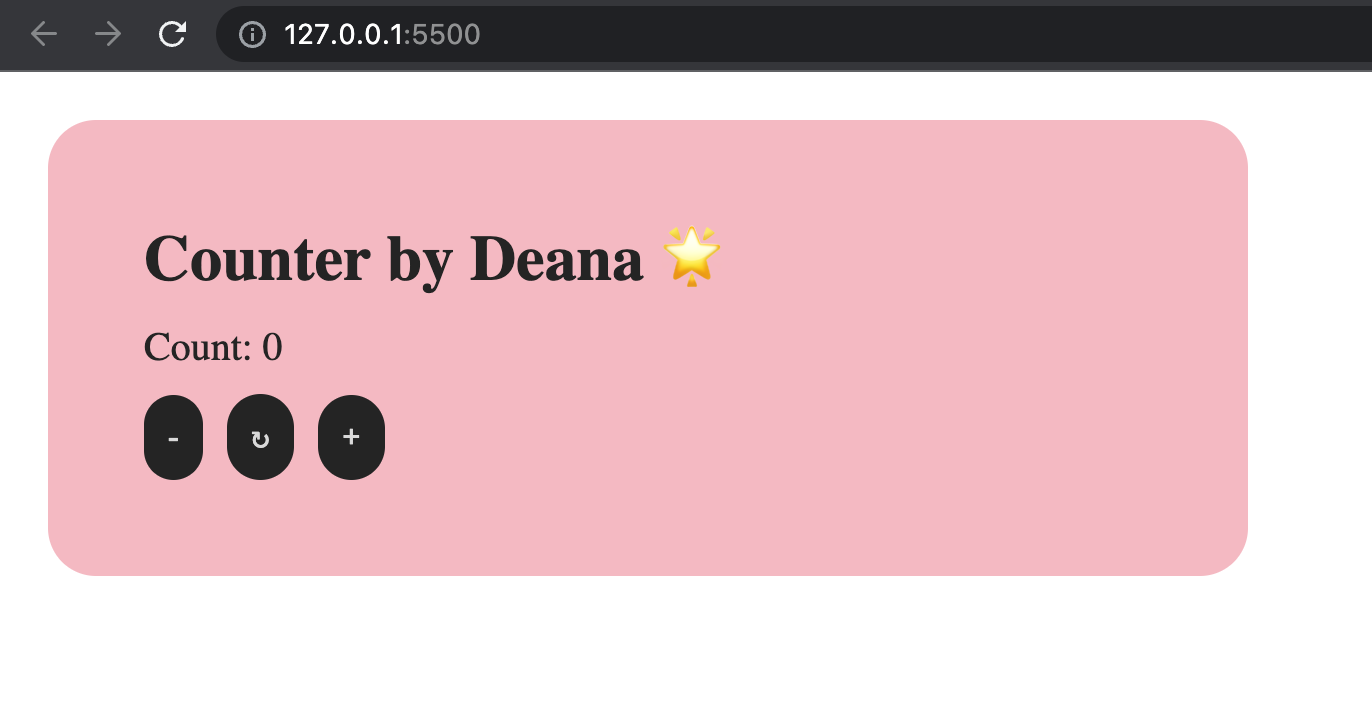
\includegraphics[width=0.8\textwidth]{Images/counter1.png}
    \caption{Counter Interface}
    \label{fig:screenshot}
\end{figure}

\begin{figure}[ht]
    \centering
    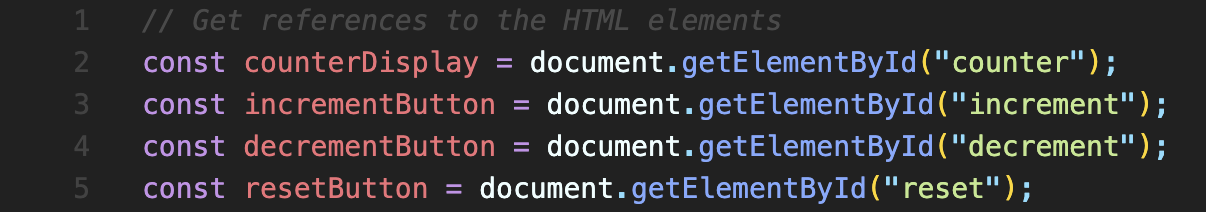
\includegraphics[width=0.8\textwidth]{Images/counter2.png}
    \caption{Accessing web-page elements}
    \label{fig:screenshot}
\end{figure}

\begin{figure}[ht]
    \centering
    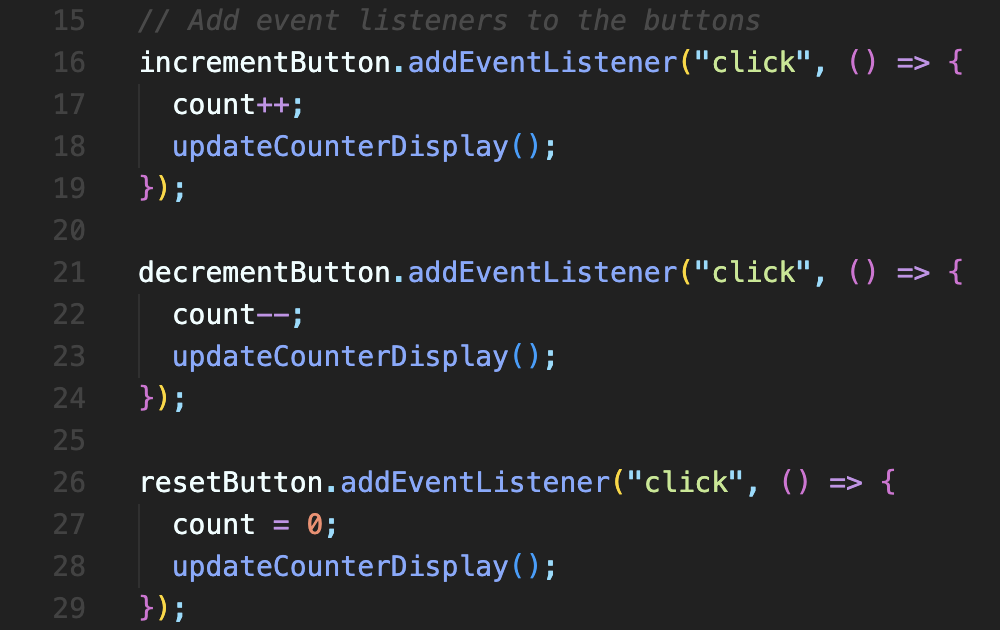
\includegraphics[width=0.8\textwidth]{Images/counter3.png}
    \caption{Event-based triggers}
    \label{fig:screenshot}
\end{figure}

%=============================================================================

\newpage

\bibliographystyle{IEEEtran}
\bibliography{main}

\end{document}
\end{report}
